\title{WED3 CheatSheet}
\author{dthoma & lroellin}
\date{August 2018}

\documentclass[a4paper, fontsize=6pt]{scrartcl}
\usepackage{multicol}
\usepackage{calc}
\usepackage{ifthen}
\usepackage[landscape]{geometry}
\usepackage{hyperref}
\usepackage{graphicx}
\usepackage{mathtools}
\usepackage{gensymb}
\usepackage{minted}
\setminted{fontsize=\footnotesize,baselinestretch=1}
\usemintedstyle{vs}
\usepackage{ragged2e} 
\usepackage[T1]{fontenc}
\usepackage[utf8]{inputenc}
\usepackage[shorthands=off,ngerman]{babel}
\usepackage{amsbsy}
\usepackage{amsfonts}
\usepackage{varwidth,pst-tree,pst-eps}
\usepackage{comment}
\usepackage{xcolor}
\usepackage{titlesec}
\usepackage{tikz}
\usetikzlibrary{shapes,arrows}

\usepackage{fontspec}

\setromanfont[
Path=fonts/Roboto/,
BoldFont=Roboto-Bold.ttf,
ItalicFont=Roboto-Italic.ttf,
BoldItalicFont=Roboto-BoldItalic.ttf
]{Roboto-Regular.ttf}
\setmonofont[
Path=fonts/Hack/,
BoldFont=Hack-Bold.ttf,
ItalicFont=Hack-Italic.ttf,
BoldItalicFont=Hack-BoldItalic.ttf
]{Hack-Regular.ttf}

\AtBeginEnvironment{minted}{%
  \renewcommand{\fcolorbox}[4][]{#4}}

%German-specific commands
%--------------------------------------
% \usepackage[german]{babel} % wegen "s => ß disabled
%--------------------------------------

\graphicspath{ {images/} }


% This sets page margins to .5 inch if using letter paper, and to 1cm
% if using A4 paper. (This probably isn't strictly necessary.)
% If using another size paper, use default 1cm margins.
\geometry{top=0.5cm,left=0.5cm,right=0.5cm,bottom=0.5cm}

% Turn off header and footer
\pagestyle{empty}
 

% Redefine section commands to use less space
\makeatletter
\renewcommand{\section}{\@startsection{section}{1}{0mm}%
    {-1ex plus -.5ex minus -.2ex}%
    {0.5ex plus .2ex}%x
    {\normalfont\large\bfseries}}
    
\renewcommand{\subsection}{\@startsection{subsection}{2}{0mm}%
    {-1explus -.5ex minus -.2ex}%
    {0.5ex plus .2ex}%
    {\normalfont\normalsize\bfseries}}
    
\renewcommand{\subsubsection}{\@startsection{subsubsection}{3}{0mm}%
    {-1ex plus -.5ex minus -.2ex}%
    {1ex plus .2ex}%
    {\normalfont\small\bfseries}}
    
\makeatother

% Define BibTeX command
\def\BibTeX{{\rm B\kern-.05em{\sc i\kern-.025em b}\kern-.08em
    T\kern-.1667em\lower.7ex\hbox{E}\kern-.125emX}}

% Don't print section numbers
%\setcounter{secnumdepth}{0}


\setlength{\parindent}{0pt}
\setlength{\parskip}{0pt plus 0.1em}

\titlespacing{\paragraph}{%
  0pt}{%              left margin
  0.5\baselineskip}{% space before (vertical)
  1em}%               space after (horizontal)

\newcommand{\css}[1]{\texttt{#1}}
\newcommand{\scss}[1]{\mintinline{scss}{#1}} % mit minted, wegen den Steuerzeichen
\newcommand{\html}[1]{\texttt{#1}}
\newcommand{\js}[1]{\texttt{#1}}
\newcommand{\csharp}[1]{\texttt{#1}}



% -----------------------------------------------------------------------

\begin{document}

\footnotesize
\begin{multicols*}{5}


% multicol parameters
% These lengths are set only within the two main columns
% \setlength{\columnseprule}{0.25pt}
\setlength{\premulticols}{1pt}
\setlength{\postmulticols}{1pt}
\setlength{\multicolsep}{1pt}
\setlength{\columnsep}{2pt}

\section{Browser-based Applications}
Today, browsers provide the required feature-set and performance to run sophisticated, web-based applications. \\
\textbf{Vorteile}: client backups werden nicht benötigt, plattform unabhängig, keine software updates für den client, Software as a Service ist möglich; \textbf{Nachteile}: Keine Hoheit über die Daten, Limitierter HW Access, Kein OS Access, Läuft überall (muss also sehr flexibel, kompatibel sein), SEO Kompatibilität (z.B. Schwerer bei SPA als bei normalen Webseiten)
\section{SPA - Single Page Application}
Ist eine Webseite, welche teile des DOMs umschreibt, statt die komplette Seite neu zu rendern. Logik wird somit teilweise vom Server auf den Client verschoben (Thin Server Architecture). Der komplette benötigte Code (HTML, JS, CSS) wird beim Aufrufen der Seite geladen oder die benötigten Ressourcen werden via Lazy Loading nachgeladen sobald benötigt und dynamisch in die Web App eingefügt.
\textbf{Vorteile}: keine Page Reloads, Fast Actions (sofortiges Feedback), bei komplexen Interaktionen vereinfacht es die Entwicklung, offline usage, schnelle page loads nach dem initialen Laden, Lazy Loading von noch nicht benötigten Komponenten. 
\textbf{Nachteile}: langer und grosser initialer Download, die Abhängigkeit von einem Frontend und dessen Updates, den Support von JS und dass gewisse Crawler damit nicht umgehen können (Lack of JS Support). Broken Back Button und Broken Reload (kann durch Libraries (z.B. durch Routing) behoben werden, funktioniert aber nicht unbedingt von Haus aus (React).
\textbf{Characteristics}: [View/Routing Layer] Plain HTML5/CSS/JS Code (no plugins), No page reloads, working back-button, bookmarkable links, [Models/Services Layer] provides offline functionality, [Data Access Layer] uses RESTful services for data access 
\textbf{Bundler}: A JavaScript bundler is a tool that puts your code and all its dependencies together in one JavaScript file (e.g. Webpack)

\subsection{React / Angular}

\textbf{React:} Freie Komponentenwahl, klein, JSX, virtual DOM
\textbf{Angular:} Framework -> kommt als "package", dependency injection, Module System

\section{Vue.js}

\textbf{Vorteile}: Lightweight, Components (Single File Components), easy to learn \textbf{Nachteile}: Small community
Braucht nur ein eingebundenes JS. Vue überwacht nur die Daten-Variabeln (data) mittels Change-Detection (Two Way Data Binding!) und "Hooks" (\js{created, mounted, updated, destroyed, beforeHook} (for every hook)). Sollte \html{\{\{\}\}} nicht gehen, kann \html{<div v-bind:id="someId" />} verwendet werden.

\textbf{Bindings:} \html{<input v-model="item.symbol" />}, \html{\{\{item.amount * find(item.symbol)\}\}} (\js{find} ist eine eigene Method), \html{<button @click="remove(item.symbol) />}.

\textbf{Direktiven} sind \html{v-on/@} für Events/modifiers, \html{v-once} (rendered only once, static content for rerenders), \html{v-html} (?), \html{v-if/v-show} (if lässt es weg, show \css{display: hidden}), \html{v-for="item in ..."}

Mit \js{watch} gibt man an, dass man bei Änderungen dieser Variable noch weitere Aktionen machen möchte. Ein Watcher auf eine Variable im Input-Feld machen und dann z.B. eine andere Liste nachladen, mit Inhalt aus diesem Input-Feld. Watch mit \js{deep} möglich, z.B. für Arrays.

\textbf{Komponenten} (ähnlich React/Angular im Sinne von: eigenständig, gekapselt). Haben einen Namen (\js{Vue.component('my-component'}) und im Minimum ein \js{template}. Dann können sie (falls registriert und gefunden etc.) mit \html{<my-component></my-component>} eingebunden werden.
\textbf{Computed properties}: Computed properties are used for caching. Example: We have a property firstname and a property lastname. We create a computed property name which consists of a function (taking no params!) returning the concatenation of the first- and lastname. 
\textbf{methods}: Methods are actual methods that can be called from the template.
\textbf{watch}: Is used to defined watchers for properties of the component. For example we could watch the value name and log the old and new name to the console (defining side effects). Is defined as a function and receives the new and the old value as params.
\textbf{computed vs watched properties:} computed properties verwenden wenn möglich. 

\begin{minted}{html}
<!DOCTYPE html> <head><meta charset="UTF-8">
<title>Hello!</title>
<script src="https://.../vue"></script>
</head><body><div id="app">
<h2 class="hello-title">Hello {{name}}!</h2></div>
<script>
var vm = new Vue({ el: '#app',
data: { name: 'Hello Vue!'}, 
created: function () {
  fetch('/spa/'+window.location.hash.substring(1))
    .then(response => response.json()) .then(body => {
this.name = body.value; });}});</script></body></html>
\end{minted}

\section{PWA - Progressive Web App}
Progressive web apps (PWAs) are web applications that are regular web pages or websites, but can appear to the user like traditional applications or native mobile applications. Benötigen einen \textbf{Service-Worker} und sind auch offline verfügbar (JS "Proxy", handlet z.B. Zugriffe online oder offline). Müssen via TLS heruntergeladen werden, und benötigen ein Manifest (mind. Properties name, short\_name, start\_url, display with a value of standalone or fullscreen, an icon at least 144x144px in png format). \textbf{Service workers}: scriptable network proxy in the web browser to manage the web/HTTP requests programmatically. \textbf{Vorteile}: Bessere User Experience, One code-base + language for mobile+desktop \textbf{Nachteile}: Yet another standard, hw access depends on standards

\section{React}

\subsection{Grundlagen}

\textbf{JSX:} React wird in JSX geschrieben, das JS mit HTML kombiniert. JSX bedingt stets einen Import von React: der Präprozessor ruft \js{React.createElement} auf. JSX ist eigentlich nur syntactic sugar. Es sind theoretisch auch mehrere Mounts auf einer Seite möglich. Möchte man eine \textbf{CSS-Klasse} als Attribut angeben, verwendet man \html{className}. Kann auch Server-side gerendert werden (\js{renderToString(<App>)}. \textbf{JSX Conditionals} \js{\{ this.state.error ? <Message negative> : <Message positive> \}} (Nur Expressions und keine Statements, da immer ein Return-Value erwartet wird.)

\textbf{Prinzipien:} Wiederverwendbarkeit, Erweiterbarkeit, Wartbarkeit, Testbarkeit, Aufgabenverteilung, Funktionale Programmierung

\textbf{Form-/Input-Handler:} Immer \js{event.preventDefault()}, sonst submittet der Browser die Form via POST/GET. 
  
\textbf{Arrays:} Elemente in einem Array brauchen einen Key, damit bei einer Positionsänderung in der Liste das bestehende Element wiederverwendet wird. Array-Index löst das Problem, aber für die Performance ist eine echte ID besser.

\textbf{Container/Presentation Komponente:} Best-Practice in der React Entwicklung ist die Trennung zwischen sogenannten Container-Komponenten und einfachen Präsentations-Komponenten (der Container lädt die Daten, die Präsentations-Komponente erhält die Daten über Props).

\textbf{Klassen-/Funktionale-Komponenten:} Hat State oder Lifecycle? Ja -> Klasse, Nein -> Funktion. Minimale funktionale Komponente mit Parameter-Objekt-Dekonstruktion \js{const HelloMessage = ({name}) => <div>Hello {name}</div>}

\textbf{Props:} Alle Parameter als \js{props} Objekt, sind immer read-only.

\subsection{State}
State einer Komponente ist immer privat und muss von dieser verwaltet werden (kann aber als Prop an Kind-Komponenten weitergegeben werden, diese State-Updates werden als Prop-Updates weitergegeben). Keine von Props abgeleiteten Daten im State speichern! Ausschliesslich mit \js{setState} ändern (sonst kann React die Änderung nicht anstossen). Möglichst wenig State verwenden!

\subsubsection{setState}
setState nimmt das Objekt entgegen und mergt es mit dem existierenden State. Nur die angegebenen Properties werden überschrieben. State Updates können zusammengefasst werden und laufen asynchron ab. Danach wird die Reconciliation aufgerufen. Man kann einen Callback angeben, der aufgerufen wird wenn die asynchrone Operation abgeschlossen ist (erst dort ist dieser State-Update aktuell).

\subsubsection{Reconciliation}
Component-Update-Mechanismus: 1. React Komponenten werden als virtueller DOM gerendert. 2. Wird der state geändert, erstellt React einen neuen virtuellen DOM 3. Alter und neuer DOM werden verglichen (Diff-Algorithmus) 4. Änderungen werden in den Browser geschrieben. Die Lifecycle Methoden werden irgendwo in diesem Prozess aufgerufen.

\subsubsection{Lifecycle}
Können in drei Phasen unterteilt werden: Mounting, Updating und Unmounting. \\
\textbf{Mounting:} 1. \js{constructor(props)} - State initialisieren 2. \js{componentWillMount()} - deprecated, constructor verwenden 3. \js{render()} 4. \js{componentDidMount()} - DOM ist aufgebaut, Guter Punkt um async Daten zu laden, setState Aufruf führt zu re-rendering \\
\textbf{Updates:}  1. \js{componentWillReceiveProps(nextProps)} - Vorschau auf die nächsten Props, davon abhängigen State hier aktualisieren 2. \js{shouldComponentUpdate(nextProps, nextState)} - wird false zurückgegeben wird render übersprungen 3. \js{componentWillUpdate(nextProps, nextState)} 4. \js{render()} 5. \js{componentDidUpdate(prevProps, prevState)} - analog zu \js{componentDidMount()}, DOM ist aktualisiert\\
\textbf{Unmounting:} 1. \js{componentWillUnmount()} - Aufräumen\\

\subsection{Testing}
\textbf{Jest:} Snapshot testing, Dom testing, Code covefe, Mocks, interaktiv.
\textbf{Enzyme:} In Kombination mit Jest erleichtert es das Schreiben von Tests (Komponenten können unterschiedlich gerendert werden).

\subsection{Redux}

Library für Statemanagement, nicht React spezifisch -> Wenn kaum Zustand existiert der von mehreren Komponenten verwendet wird lohnt sich der Redux-Overhead nicht!

\textbf{Ohne Redux:} Daten immer mitgeben ist mühsam, Zustand in Applikation verteilt, Calls zum Backend verteilt, Brauchen mehrere Komponenten dieselben Daten, muss der Zustand über einen gemeinsamen Parent verschoben werden.

\textbf{Mit Redux:} Bessere Übersicht, da Zustand an einer Stelle, Einfacheres Zustandsdebugging,  Einfachere React-Komponenten

\subsubsection{State}
Der Store ist ein Tree von State-Objekten (single source of truth) und ist immutable  -> Veränderung führt zu neuem Tree.

React-Redux Library bietet \js{connect(mapStateToProps: (state) => props, mapDispatchToProps: (dispatch) => props})(TodoListComponent) an. Das Resultat ist eine React-Komponente, die aber noch der React-Komponentenhierarchie bekannt gemacht werden muss.

\textbf{Change:} 1. Action wird an den Store gesendet / dispatched. 2. Der Store benutzt sogenannte Reducer-Funktionen um den State t+1 zu erstellen. 3. Reducer erstellt einen neuen State Tree aufgrund der Action (auch Reducer sind pure Funktionen, haben also keine Seiteneffekte).

\textbf{mapStateToProps:} Für die Komponente benötigte Props aus dem State-Tree auslesen, Properties des Rückgabeobjekts werden der React-Komponente von der connect-Methode als Props gesetzt.

\textbf{mapDispatchToProps:} Mit der Dispatch-Funktion können Actions an den Store dispatched werden. Properties des Rückgabeobjekts werden der Komponente als Props gesetzt.

\textbf{Reducer:} Reducer ist immer nur für einen Teil (Slice) des State-Trees zuständig. Mehrere Reducer werden dann zu einem Root-Reducer kombiniert.

\subsection{React Router}
Komponentenbibliothek die es erlaubt, Komponenten anzuzeigen oder zu verstecken abhängig von der URL. Supported auch Server Side Rendering, Animated Transitions, Redux Integration.

\begin{minted}{html}
<Router>
  <Route exact path="/" component={Home} />
</Router>
\end{minted}

Alle Routen müssen Teil des Routers sein, Component Home wird nur gerendert, wenn der path (hier exakt) matched, App-interne Links verwenden (nicht \html{<a>} sondern \html{<Link>}). Für Redirects kann auch ein \html{<Redirect>} geändert werden.

\section{Angular}

Framework. TypeScript based, tries to reduce boilerplate code, dependency injection, RXjs, easier binding, covers a wide range (template to data-services). -> Angular comes with a lot of features, but adds another abstraction and complexity level.

\textbf{Names:} AngularJS (v1), Angular (2+), 3 has been left out, v6 is current

\subsection{Architecture}
\textbf{Modules:} A cohesive block of code dedicated to closely related set of capabilities.

\textbf{Directives:} Provides instructions to transform the DOM. (e.g. ng-if, ng-for)

\textbf{Components:} A component is a \textit{directive-with-a-template}; it controls a section of the view.

\textbf{Templates:} A template is a form of HTML that tells Angular how to render the component.

\textbf{Metadata:} Metadata describes a class and tells Angular how to process it.

\textbf{Services:} Provide logic of any value, function, or feature that your application needs.

\subsection{Modules}

Each ts-file represents exactly one TypeScript module. Multiple TypeScript modules within a directory can be re-exported within a single index.ts file (this is then called barrel file). Angular Modules behave differently to TypeScript (and ES6) modules. An Angular module is a logical block of multiple modules linked together (may even include subfolders etc.). Every app has at least one Angular module, the \js{root} Module (a.k.a. \js{app} Module). To bootstrap the application, this module is launched.

\subsubsection{\js{@NgModule}}
\textbf{\js{declarations: [ Type1, Type2, Type3, ]}} The view classes that belong to this module. Angular has three kinds of view classes: \textit{components}, \textit{directives} and \textit{pipes}.\\
\textbf{\js{exports: [ Type1, Type2, ..., Module1, Module2 ]}} The subset of declarations that should be visible and usable in the component templates of other modules. Can re-export other modules, which are automatically included when importing this module.\\
\textbf{\js{imports: [ Module1, Module3, ]}} Specifies the modules which exports/providers should be imported into this module.\\
\textbf{\js{providers: [ Provider1, Provider2, ]}} Creators of services that this module contributes to the global collection of services (Dependency Injection Container); they become accessible in all parts of the app.\\
\textbf{\js{bootstrap: [Component]}} Only the root module should set this property. The main application view, called the root component.

\subsubsection{Imports}

\textbf{Default Imports}: If you import a whole module into your module, all Components, Pipes, Directives from the given \js{ForeignModule} are imported (everything specified in exports of this module). Providers are registered into the current DI container, if registration not done yet.\\
\textbf{forRoot(config?) - Für Eager Loading}: Must be implemented as a static method in the module class by developer himself.  It returns an object with a \js{providers} property and a \js{ngModule property}. Nur im Root Module (App Module) Module so importieren. Injected Services in den Root DI Container. Services sind so konfigurierbar. \js{imports: [ForeignModule.forRoot()]}. Declare providers in NgModule or .forRoot() but never in both!\\
\textbf{forChild(config?) - Für Lazy Loading}: Must be implemented as a static method in the module class by developer himself. It returns an object with a providers property and a ngModule property. It’s nearly the same as a default import but allows you to configure services for the current Module level.
ForChild is used when we want to deliver a provider that is visible only to the "children" modules of our module, in case they are lazy loaded. Injected Services in den eigenen DI Container. \js{imports: [ForeignModule.forChild()]}

\textbf{Provider Priority List 1.} \js{providers} defined in App/Root Module, 2. \js{providers} defined in \js{forRoot()} definitions, 3. \js{providers} defined in imported Module definitions.

\subsubsection{Module Types}

\textbf{Root / App Module} Provides the entry point (bootstrap component) for the app (Provides main view, doesn’t export anything, called \js{AppModule}, imports \js{BrowserModule}).
\textbf{Feature Modules} Specifies clear boundaries between the application features. Can be categorised into more granular module types. Routing Modules and Lazy Modules are subtypes. Lazy Modules are loaded on-demand and have their own DI container.
\textbf{Shared Modules} Hold common components/directives/pipes of the app and shares them with the feature modules.
\textbf{Core Modules} Keep the Root Module clean. Contains components/directives/pipes used by the Root Module. Additionally, globally used services can be declared here. Should only be imported by the root module.


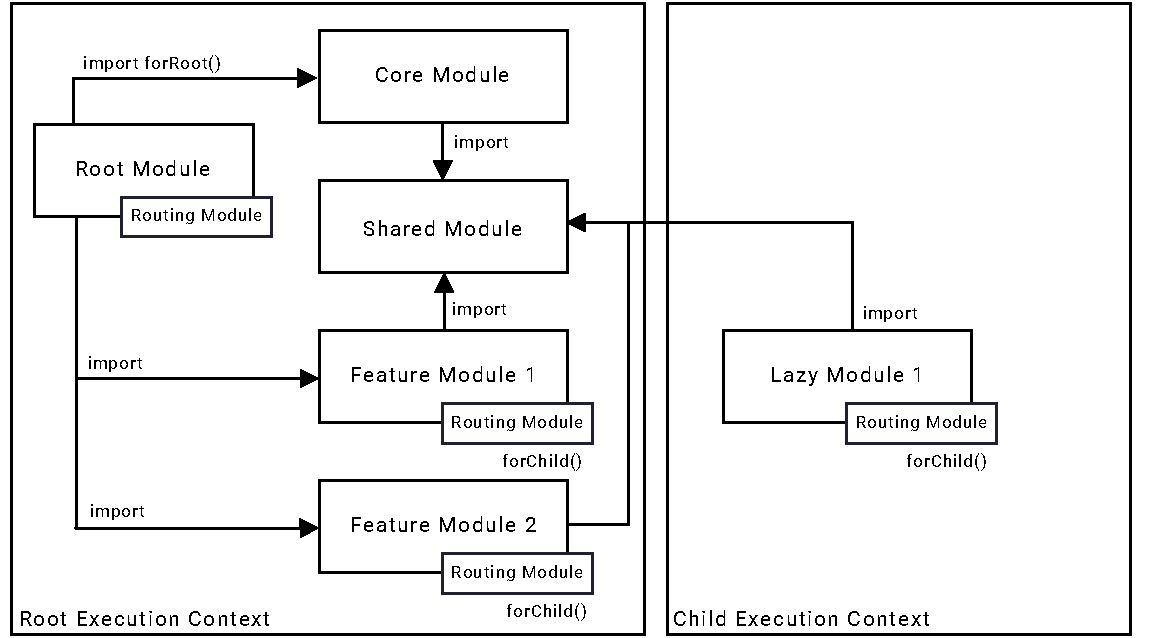
\includegraphics[scale=0.27]{angular-modules.pdf}

\subsection{Views (UI)/Routing}

\subsubsection{View Encapsulation}
Bei der View Encapsulation geht es darum, wie und ob die Implementation der Komponenten im DOM verborgen wird. Es gibt drei verschiedenen Werte, welche gesetzt werden können: ViewEncapsulation.[None, Emulated, Native]. None: No Shadow DOM at all. Therefore, also no style encapsulation. Emulated: No Shadow DOM but style encapsulation emulation. Native: Native Shadow DOM. Sie hat keinen Einfluss auf die Change Detection.
\textbf{Shadow DOM}: A shadow dom is a browser feature which hides the implementation of a component in a additional "hidden" DOM which is attached to the regular DOM using a Shadow root node. For example. The <mycomponent> would be visible in the browser only. Styling and structure of this would be hidden. Need to activate "show shadow dom" in the browser to see implementation (Example of this: <video> tag in HTML). 

\subsubsection{Components}

Components support the view and provide the application logic for the view. A component consists of exactly one view, and a \js{selector} is used to embed this component into another view (HTML tag or CSS selector). Also specifies an HTML \js{templateUrl} and CSS \js{styleUrls}. Simplified, a component consists of logic in Typescript, a view (template) in HTML and styles in CSS. The components must be declared within the containing module.

\textbf{Component Lifecycle:} \js{constructor}, \js{ngOnChanges}, \js{ngOnInit}, \js{ngDoCheck}, (\js{ngAfterContentInit}, \js{ngAfterContentChecked}, \js{ngAfterViewInit}, \js{ngAfterViewChecked}, these are mainly for control developers to handle their sub components), \js{ngOnDestroy}. These can be overwritten. \js{ngOnInit} (hydration) initialize before Angular displays the first data-bound properties: setup the component and initially fetch data. \js{ngOnDestroy} cleanup just before Angular destroys it: detach event handlers to avoid memory leaks.

\textbf{Component Transclusion} are the child components inside your component (like React's \js{children}). Can be included with \js{ng-content} (single-slot) and there's a multi-slot variant.

\textbf{Component Tree} The result of nested components is a component tree. It’s then used for things like Hierarchical DI, Change Detection or View Encapsulation. A provider can be re-configured at multiple tree levels (at their child injector). The first provider encountered in the tree wins (from bottom to top, from the component to the root). An intermediate injector may intercept a request for a service (=proxy). If providers at the top level are specified, the injector tree appears to be flat.

\subsubsection{Change Detection}

Application state change can be caused by these asynchronous \textbf{invocations}: 1. Events (click, submit, ...), 2. XHR (fetching data from a remote server) 3. timers (\js{setTimeout, setInterval}. Each component has its own change detector. They compose a parallel change detector tree. Change detection is always performed from top to bottom for every single component. Jeder Component kann seinen eigenen Change Detector anfordern (DI). 

A \textbf{zone} monkey-patches global asynchronous operations. Zones represent a VM (a set of patches). Zones provide hooks to listen for patched function invocations. Angular forks the global zone to \js{ngZone}. ngZone defines custom events: \textbf{\js{onTurnStart()}} notifies subscribers \textbf{just before} Angular's event turn starts. Emits an event once per browser task that is handled by Angular. \textbf{\js{onTurnDone()}} notifies subscribers \textbf{immediately after Angular's zone is done processing} the current turn and any micro tasks scheduled from that turn. \textbf{\js{onEventDone()}} notifies subscribers \textbf{immediately after the final \js{onTurnDone()} callback} before ending VM event. Useful for testing, to validate application state.

Every Angular API call must be executed within the ngZone which can get bad performance-wise. To run a long calculation without Angular API calls, you can use \js{NgZone.runOutsideAngular()}

Angular applies two Change detection runs. The first applies the changes, the second checks the bindings against unknown changes. An error is thrown if the bound value differs.

OnPush can be specified in the metadata of a component, which limits the change detection to stop at the current component level, if there are no @Input value changes. If there is no @Input change detection is skipped on the complete subtree. However, you can still force a single run with \js{markForCheck}.

\subsubsection{Templates}

\textbf{Binding}

\textbf{Property Binding} one-way from data source to view target: \js{\{\{counter.team\}\}}, \html{<img [attr.alt]="counter.team"}.
\textbf{Event Binding} one way call from view target to data source: \html{<button (click)="counter.eventHandler(\$event)">}. \textbf{Property and Update Event Binding} two-way: \html{<input type="text" [(ngModel)]="counter.team"} (Banana in a box)

\textbf{Targets}
Binding to targets must be declared as \js{@Input} (fires bindable events) or \js{@Output} (consumes bindable values) in your component. \html{<wed-navigation (click)="..." [title]="..." />}. Im Component dann \js{@Output() click: EventEmitter<any>; @Input() title: string }

\textbf{Directives}

Like a component, but has no template. \textbf{Structural Directives} modify the DOM. \textbf{Attribute Directives} alter the behavior of an element. \textbf{Structural Directives} start with an asterisk (\js{*}), e.g. \html{<div *ngFor="let element of elements">...</div>} \textbf{Attribute Directives} are applied to a host element as an attribute, e.g. \html{<div [style.font-size]="isSpecial ? 'x-large' : 'smaller'"}. Asterisk is syntactic sugar for (two stages): \html{*directive="..."} is translated to (1) a template attribute \html{ng-template="directive ..."} and then to a (2) \html{<ng-template>}

\textbf{Template Reference Variable}

References a DOM element within a template. Can also be a reference to an Angular component or directive, reference variables can be used anywhere in the template.

\begin{minted}{html}
<input placeholder="phone number" #phone>
<button (click)=callPhone(phone.value)">Call</button>
\end{minted}

\textbf{Safe Navigation Operator} When \js{x} may be null but could have an attribute \js{name}, you can navigate with \js{x?.name}. This will either display the value, or will be displayed blank. Useful while loading!

\subsubsection{Forms}

1. Template-driven forms, which put the validation logic in HTML (but less TS code) 2. reactive (model-driven) forms. Designed for daily use, with async validation, and testable validation logic. \textbf{Lecture is only about template-driven!}. \textbf{Shortcut} if you have an \html{<input name="xyz">} and a property (on the same component) called \js{xyz}, you can simply use \html{<input type="text" ... name="xyz" ngModel>} and it will automatically map (two-way).\\To test, you can check a \js{valid} property on the object you reference. Use \html{(ngSubmit)="doLogin(...)"} to submit. 

\subsubsection{Routing}

The served \html{index.html} needs to include a base href (\html{<base href="/"}) for the router to work out, what page to display. This will be used as the static part of the URL. The top-most router must be registered with \js{forRoot()}. Always use \html{<a routerLink="/bla">}! Route definitions may also include variables, e.g. \js{'hero/:id'}, wildcards, and a \js{redirectTo} property. Routes are matched in their order! There are guards, e.g. \js{canLoad}. Don't use \js{canActivate}, since this would always load it, even though the guards disallows it.

Routers have a list of defined routes and a router outlet. From the path, they then decide what route's content to display in the outlet. Also, a route may include another router component. In this case, the sub-router \textbf{only gets the not-yet-consumed part}. 

To achieve \textbf{lazy loading}, instead of \js{path: 'bla', component: BlaComponent}, use \js{path: 'bla', loadChildren: 'app/lazy/lazy.module\#LazyModule}

\subsubsection{Pipes}

Pipes are a good choice for small transformations. \textbf{Pure} Pipes are pure by default -> functions without side effects. Ignores changes within composite objects/values -> restrictive but fast. \textbf{Impure} Impure pipes are executed on every component change detection cycle (this means every keystroke, mouse-move or other event -> long-running impure pipes could destroy the user experience -> to reduce processing time, caching is often seen inside impure pipes. \textbf{Filter / OrderBy Pipes} don’t exist because of bad performance. -> Move filtering and sorting logic into the component itself.


\subsection{Models / Services}

\subsubsection{Services}

Provides stuff that your application needs, e.g. logging service, data service, ... Angular uses DI to provide new components with the services they need => the services must be registered within the DI container.

Service must be marked \js{@Injectable} and registered in the modules \js{providers}. Then, you need to have a (e.g.) \js{contructor (cService CounterService)} in your component, where the Angular injector will automatically inject the service (\js{CounterService} in this case, based on the type). 

\textbf{Communicate with UI}

Add an \js{EventEmitter} to service. Whenever you (e.g.) reload stuff, emit this event. In \js{ngOnInit} of the component, subscribe to the service's event (and declare a callback in case it fires) and unsubscribe in \js{ngOnDestroy}.

\subsection{Data Access}

\subsubsection{\js{HttpClient}}

Provides an HTTP client that works with Observables. There are hot observables (sequence of events, shared among all subscribers, like mouse clicks) and cold observables (started on request, e.g. async web request, not shared, automatically closed after task is finished). The \js{subscribe} method on an observable takes \js{onNext, onError} and \js{onComplete}. Angular automatically handles the response as JSON! It is possible to develop custom interceptors to HTTP requests, e.g. to inject an Authorization header on every request. It needs to go into the DI container, but then they're \textit{automatically} hooked. You just send an HttpRequest and the interceptor will get it automatically.

% Examples: Angular Basics 2, Pages 26-28, falls nötig

\section{ASP.NET}

Enterprise Framework, Kompilierbare Sprache (C\#), komplett neue Entwicklung, Cross-Plattform kompatibel (Linux, Mac, Windows)\\
\textbf{Convention over Configuration:} (also known as coding by convention) is a software design paradigm which seeks to decrease the number of decisions that developers need to make, gaining simplicity, and not necessarily losing flexibility.\\
\textbf{Multi-Threading:} ASP.NET besitzt einen Thread Pool (Grösse konfigurierbar) und wählt für jeden Request einen Thread aus diesem Pool aus. Thread ist blockiert bis Request beendet (vorzeitig freigeben mittels async/await). Da ASP.NET für jeden Request einen neuen Service/Controller instanziert, sollten darin keine geteilten Daten gespeichert werden.\\
\textbf{Front-Controller:} Ein Front-Controller ist ein Entry Point in die Applikation und handlet das \textbf{Routing}. Er wird den Page Controllern vorgeschaltet und leitet die entsprechenden Requests an den Controller weiter.\\
\textbf{ActionResult:} Erzeugt ein Resultat, welches zum Client gesendet wird. Mögliche Resultate: View, Partial View, Content, Empty, File, StatusCode, Json, Redirect/RedirectToRoute/RedirectToAction \\
\subsection{Middlewares:} Jeder Request durchläuft einen Stack von Middlewares.
Registriert eine neue Middleware
\begin{minted}{csharp}
app.Use(async (context, next) => { 
Debug.WriteLine("Handling request");
await next.Invoke();
Debug.WriteLine("Finished handling request.");
});
\end{minted}
App.Use -> "normale" Middleware, App.Run -> Terminierende Middleware (kein Next aufruf), App.Map -> maps a request path to a sub-request pipeline.

Eigene Middleware:  1. Param vom Konstruktor ist nachfolgende Middleware. Weitere Parameter werden vom Dependency Container aufgelöst

\subsection{Razor - Template Engine}
\subsubsection{Tag Helper}
Ermöglichen es CSharp Code an HTML Tags zu binden. Bsp. E-Mail Tag soll durch einen Link Tag ersetzt werden:
\begin{minted}{csharp}
<email mail-for="support@example.com"></email>
// wird zu
<a href="mailto:support@example.com">
support@example.com</a>
// Tag Helper erstellen
public class EmailTagHelper : TagHelper {
public string MailFor { get; set; }
public override void Process(TagHelperContext context, 
TagHelperOutput output) {
output.TagName = "a"; 
Attributes.SetAttribute("href", "mailto:" + MailFor); 
output.Content.SetContent(MailFor);
} }
// Helper im File _ViewImports.cshtml registrieren:
@addTagHelper*, Microsoft.AspNetCore.Mvc.TagHelpers
@addTagHelper*, Pizza
\end{minted}
\subsubsection{Layout}
Layout File: Definiert das generelle Layout für die Applikation. Definiert Sections (Placeholders), welche von der Content Page abgefüllt werden können/müssen.\\
\textbf{@RenderBody:} Definiert den Platz, an welchem die Content Page gerendert wird.\\
\textbf{@RenderSection:} Definiert eine Sektion, in welche die Content Page ihren Content platzieren kann.

\begin{minted}{csharp}
// Default Layout überschreiben
@{Layout = "~/Views/Shared/_Layout.cshtml";}
// Sections
@section Scripts {Scripts.Render("~/bundles/jqueryval")}
\end{minted}
\subsubsection{MVC Razor Datentransfer}
\textbf{Ohne Typensicherheit:} \textbf{Per Action} - ViewData/ViewBag (Wrapper für ViewData) \textbf{Per Request (überleben einen Redirect)} - TempData (Session notwendig)\\
\textbf{Mit Typensicherheit:} Model

\subsubsection{Service Injection im Razor File}
\begin{minted}{csharp}
@inject DataService DataService; 
@{<ul>
@foreach(var data in DataService.GetData()) {
  <li>@data</li> }
</ul> }
\end{minted}

\subsection{Session}
\begin{minted}{csharp}
// Assuming Config is done (app.UseSession()), 
// this is the usage
public IActionResult Index() {
var value = (
  HttpContext.Session.GetInt32(SessionKey) ?? 0) + 1; 
HttpContext.Session.SetInt32(SessionKey, value);
return Content($"Dein {value}-xter Besuch");}
\end{minted}

\subsection{Model Validierung}

\textbf{Model} Die Klassen/Attribute mit z.B. \csharp{[StringLength(60, MinimumLength = 3)]} annotieren (kombinierbar).\\
\textbf{Razor} ausserhalb der Form Group \html{<div asp-validation-summary="ModelOnly" class="text-danger" />}, beim einzelnen Feld \html{<span asp-validation-for="Name" class="text-danger" />}. Es fehlen noch Scripts, die in der Scripts-Section mit \html{@{await Html.RenderPartialAsync("\_ValidationScriptsPartial");}} eingefügt werden können.\\
\textbf{Server-seitig} \csharp{if (ModelState.IsValid)}

\subsection{Authentifizierung}
Folgende Klassen können über DI injected werden. Die Konfiguration dieser erfolgt beim Registrieren:\\
\textbf{UserManager<ApplicationUser>:} Verantwortlich für die Verwaltung von Benutzer \\
\textbf{RoleManager<IdentityRole>:} Verantwortlich für die Verwalten von Rollen \\
\textbf{IAuthorizationService:} Verantwortlich für die Validation von Policies \\
\textbf{SignInManager:} Verantwortlich für das Einloggen \\

\begin{minted}{csharp}
services.AddIdentity<ApplicationUser, IdentityRole>(
options => {options.Password.RequireDigit = false;
})
\end{minted}

Mit \csharp{[Authorize]} auf der Action kann ich automatisch überprüfen, dass der User authentifiziert (!) ist. Ansonsten erfolgt ein 401 zur Login-Page.

\textbf{Was ist ein Claim?} Ein Statement über einen User ausgestellt vom Identity Provider (e.g. User1 hat die Admin Rolle).

\subsection{Autorisierung}
Was darf ich?
\textbf{Policies} ermöglichen komplexere Regeln zu definieren

\subsection{Unit Testing}
\begin{minted}{csharp}
public class HomeControllerTest{
[Fact]
public void TestName() {
var settingUpper = new NameSettings();
var settingLower = new NameSettings() { 
LetterCase = "lower" }; 
var name = ("Pizza Shop - The Best!").ToUpper();
var controller = new HomeController();
Assert.Equal(name, 
((ContentResult) controller.Name(settingUpper)).Content); 
Assert.NotEqual(name, 
((ContentResult) controller.Name(settingLower)).Content);
}}
\end{minted}

\subsection{Init Data/App Secrets}
Ermöglicht es «Secrets» in ein separaten File zu persistieren (PW, Verbindungsdaten).\\
\textbf{Wert setzen:} dotnet user-secrets set admin-pwd 123456
\textbf{Wert nutzen:}
\begin{minted}{csharp}
// Config
if (env.IsDevelopment()) {
builder.AddUserSecrets<Startup>();
}
// Usage
app.ApplicationServices.GetService<DataService>()
.EnsureData(Configuration["admin-pwd"]);
\end{minted}

\subsection{Swagger}
Vorteile von Swagger: Client und Server generieren, Swagger-API Doku generieren, Comments können als XML exportiert werden und für die API-Doku verwendet werden. Auto-Generierung mit \csharp{services.AddSwaggerGen()} aktivieren, folglich unter \html{/swagger} erreichbar. Möglichkeit API zu testen. API berücksichtigt C\# Funktionsdokumentations header (Javadoc).

\subsection{HATEOAS}
With HATEOAS, a client interacts with a network application whose application servers provide information dynamically through hypermedia. A REST client needs little to no prior knowledge about how to interact with an application or server beyond a generic understanding of hypermedia. 

\subsection{JSON Web Token (JWT)}
\textbf{Aufbau:} Header, Payload, Signatur\\
\textbf{Header:} beschreibt den Signatur- und/oder Verschlüsselungsalgorithmus und den Token-Typ. Die Daten werden im JSON-Format abgelegt und Base64-kodiert.
\textbf{Payload:} Daten werden mit algorithmus aus header signiert. Als Payload wird das JSON-Objekt bezeichnet, das aus einer “beliebigen” Anzahl von Key/Value-Paaren besteht. Diese Key/Value-Paare werden ”Claims” genannt. Der Payload  wird ebenfalls Base64-kodiert.
\textbf{Signatur:} Die Signatur wird aus dem Header und der Payload berechnet. 
\begin{minted}{javascript}
content = base64UrlEncode(header) + "." + 
base64UrlEncode(payload);
signature = HMACSHA256(content, secret);
\end{minted}
\textbf{Übertragung:} Ein JWT wird im HTTP Header als \texttt{Authorization: Bearer <token>} eingefügt. Base64 encoded\\
\textbf{Sicherheit:} JWTs sollten via HTTPS übermittelt werden, da man ansonsten das Token von einem anderen Client stehlen könnte.
\subsection{Dependency Injection}
\textbf{Lifetime:} \textbf{Transient} - Transient Lifetime Services are created each time they are requested. This works best for lightweight, stateless services. \textbf{Scoped} - Scoped Lifetime Services are created once per request, \textbf{Singleton} - Are created the first time they are requested (or when ConfigureServices is run if you specify an instance there) and every subsequent request will use this instance.\\
\textbf{Captive Dependency Problematik:} A “captive dependency” occurs when a component intended to live for a short amount of time gets held by a component that lives for a long time. Daher folgende Regel: Komponenten dürfen sich nur durch Komponenten mit gleicher oder längerer Lebensdauer injecten lassen. Kann z.B. bei DB zugriff zu Problemen führen, da die Session länger lebt als nötig und Vebrindungen blockiert

\subsection{Security - anti-forgery tokens}
The \texttt{\_\_RequestVerificationToken} is used to prevent CSRF. In ASP.NET Core, the tokens are added to your forms automatically when you use the asp-* tag helpers. Adding the form field is just one part of the requirement, you also need to actually check that the tokens are valid on the server side. You can do this by decorating your controller actions with the \textbf{[ValidateAntiForgeryToken]} attribute. You'll need to add it to all of your POST actions to properly protect your application. \textbf{Automatically validating all appropriate actions:} The [AutoValidateAntiForgeryToken] attribute works identically to the [ValidateAntiForgeryToken] attribute, except that it ignores "safe" methods like GET and HEAD. Adding the attribute to your application is simple - just add it to the global filters collection in your Startup class, when calling \csharp{AddMvc(options) => { options.Filters.Add(new AutoValidateAntiforgeryTokenAttribute()); }}

\subsection{Form Handling (manuell)}

\html{firstName} als \html{name} im Input entspricht dem Parameter \csharp{firstName}

\begin{minted}{html}
<form method="POST"><input name="firstName" />
<input type="submit" /></form>
\end{minted}

\begin{minted}{csharp}
public class FormController : Controller {
  [HttpGet]
  public IActionResult Index() {
    return View();}
  [HttpPost]
  public IActionResult Index(string firstName) {
      return Content($"Hello {firstName}");} 
  [HttpPost]
  [Route("/index2"]
  public IActionResult Index2() {}}
\end{minted}

\subsection{Form Handling (Model)}

\begin{minted}{csharp}
public class FormModel {
  public string FirstName { get; set; }}
\end{minted}

\begin{minted}{html}
@model FormModel
<form asp-action="Index" asp-controller="Form">
  <label asp-for="FirstName"></label>
  <input asp-for="FirstName" placeholder="..."/>
  <input type="submit" />
</form>
\end{minted}

\begin{minted}{csharp}
[HttpPost, ValidateAntiForgeryToken]
public IActionResult Index(FormModel model) {
  return Content($"Hello {model.FirstName}");}
\end{minted}


\subsection{Example APP}
\subsection{Startup.cs}
\begin{minted}{csharp}
public class Startup {
public Startup(IConfiguration configuration) {
Configuration = configuration;}
  public IConfiguration Configuration { get; }
  public void ConfigureServices(
    IServiceCollection services) {
  services.AddMvc();
  services.AddTransient<IBmiService, BmiService>();}
  
public void Configure(IApplicationBuilder app, 
    IHostingEnvironment env) {
  app.UseStaticFiles();
  app.UseMvc(routes => {
  routes.MapRoute(
    name: "default",
    template: "{controller=Home}/{action=Index}/{id?}");
  });}}
\end{minted}

\subsubsection{Controllers/Controller.cs}
\begin{minted}{csharp}
namespace Uebung.Controllers {
public class HomeController : Controller {
private readonly IBmiService _bmiService;
public HomeController(IBmiService bmiService) 
  =>_bmiService = bmiService;
public IActionResult Index() => View();
public IActionResult Bmi() => View();

[HttpPost]
public IActionResult Bmi(Bmi data) {
  if (ModelState.IsValid) {
    ViewBag.Value = _bmiService.Calculcate(data);
    return PartialView("Bmi");}
  return Content("Komische Daten");
}
public IActionResult Bmi2(Bmi data) {
  ViewBag.Value = _bmiService.Calculcate(data);
  return View("Bmi");}}}
\end{minted}

\subsubsection{Models/Bmi.cs}
\begin{minted}{csharp}
namespace Uebung.Models {
public class Bmi {
[Range(0, 300)]
[Display(Name = "Gewicht in kg")]
public double Weight { get; set; }
[RegularExpression(@"^[0-9]{4}\$", ErrorMessage = "E!!")]
public double Height { get; set; }}}
\end{minted}

\subsubsection{Services/BmiService.cs}
\begin{minted}{csharp}
namespace Uebung.Services {
public interface IBmiService {
double Calculcate(Bmi data);}
public class BmiService : IBmiService {
public double Calculcate(Bmi data) {
  return Math.Round(data.Weight/Math.Pow(
    (data.Height/100), 2),2);}}}
\end{minted}

\subsubsection{Views/Home/Index.cshtml}
\begin{minted}{csharp}
@model Bmi
@{ ViewData["Title"] = "Home Page"; }
<form asp-action="Bmi" data-ajax="true" 
data-ajax-method="POST" data-ajax-mode="replace"
data-ajax-update="#result">
    <label asp-for="Height"></label>
    <input asp-for="Height" />
    <label asp-for="Weight"></label>
    <input asp-for="Weight" />
    <input type="submit" value="Rechnen!"/>
</form>
<div id="result"></div>
@section Scripts{
<!-- script jquery.unobtrusive-ajax.min.js -->}
\end{minted}

\subsection{EchoServer}
\subsubsection{Startup.cs}
\begin{minted}{csharp}
/.../
public void ConfigureServices(
  IServiceCollection services) { 
services.AddSession(
options => 
  {options.IdleTimeout = TimeSpan.FromMinutes(15); });
services.AddMvc();}

public void Configure(IApplicationBuilder app, 
IHostingEnvironment env) {
app.UseSession();
app.UseStaticFiles();
app.UseMvc(routes => {
routes.MapRoute(
name: "echo_to_index",
template: "echo",
defaults: new { controller = "Home", action = "Index" });
routes.MapRoute(
name: "default",
template: "{controller=Home}/{action=Index}/{id?}");});}
\end{minted}

\subsubsection{Index.cshtml}
\begin{minted}{csharp}
@model Echo.Models.EchoModel
<form method="POST" asp-action="Index"asp-controller="Home">
<label asp-for="Echo">Text</label>
<input type="text" asp-for="Echo"/>
<input type="submit"/>
</form>
\end{minted}

\subsubsection{EchoResult.cshtml}
\begin{minted}{csharp}
@{ string echoText = ViewBag.echoText;}
<p>Deine Worte: @echoText</p>
@Html.ActionLink("Zurück", "Index", "Home", null, null)
\end{minted}

\subsubsection{EchoModel.cs}
\begin{minted}{csharp}
public class EchoModel {
public String Echo {get; set;}}
\end{minted}

\subsubsection{HomeController.cs}
\begin{minted}{csharp}
namespace Echo.Controllers {
public class HomeController : Controller {
public IActionResult Index() { return View();}

[HttpPost]
public IActionResult Index(EchoModel model){
TempData["text"] = model.Echo != null ? model.Echo : "----";
return RedirectToAction("EchoResult");}

public IActionResult EchoResult() {
ViewBag.echoText = TempData["text"];
return View();}}}
\end{minted}

\section{Grafik}

\subsection{SVG}

Default size: 300x150px. Koordinaten starten oben links und gehen nach rechts (x positiv) und nach unten (y positiv). Im Browser muss ein SVG eine Grösse und eine Breite haben! Mit der Viewbox kann angegeben werden, was davon dargestellt werden soll (die Width/Height kann grösser sein, das wird unsichtbar gezeichnet. Wir geben an, welchen Ausschnitt wir wollen). SVG können als \html{<object data=".svg" />} oder als Bild (\html{img}) eingefügt werden. Als Bild verlieren sie die Interaktionsmöglichkeiten. Wenn die Viewbox angegeben wird, kann mit \html{preserveAspectRatio} angegeben werden, wie das Bild dargestellt wird wenn es verzerrt würde. SVG erlaubt CSS!

Polyline vs. Polygon: Polyline ist ein Zug von X-Y-Punkte welche mit einer Linie verbunden wird. End-/Startpunkt können unterschiedlich sein. Das Polygon stellt sicher, dass die Geometrie abgeschlossen ist.

\subsection{Canvas}

Vorteile: Performance, JS, Browser Support, WebGL. Nachteile: Accessibility, Event Handling. Width/Height auch hier nötig!
Default size: 320x150px
Context ist die Leinwand. Holt man sich mit \js{const context = painting.getContext("2D")} (oder \js{"webgl"}). Der Context hält sich einen State (Farbe, Font, Stroke, Transforms, ...). Man kann den Context (mit Stack!) speichern \js{save()} und restoren \js{restore()}

Canvas kennt nur 2 primitive Shapes, Rectangle und Path. Path erstellen: (1) \js{beginPath} erstellen, (2) \js{arc/moveTo/lineTo/...} zusammen bauen, (3) Optional \js{closePath} schliessen, (4) \js{stroke/fill} Render-Variante auswählen.

\subsection{2D-Techniken}

\textbf{Double Buffering} Canvas 1 darstellen, Canvas 2 neu zeichnen. Canvas 1 und zwei austauschen. HTML Canvas macht das meistens automatisch! \textbf{Pre-Rendering} in einem nicht sichtbaren Bereich zeichnen, und dann diesen Canvas als ganzes auf dem sichtbaren Canvas zeichnen. \textbf{Layering} Canvas 2D kennt keine Layers. Lösung: 2 Canvas übereinander positionieren. \textbf{Animationen}: Bei Canvas müssen animationen selbst erstellt werden: 1. (Optional) Position von Objekten bestimmen, 2. Canvas löschen, 3.Canvas neu zeichnen, 4. Timer neu stellen. 
Anstatt den Timer selber zu stellen, sollte man mit \js{window.requestAnimationFrame(callback(timestamp))} arbeiten. Der Browser kontrolliert diese Methode, und ruft sie z.B: im Hintergrund nicht auf. Dort nicht mit Ticks arbeiten! Das Callback erhält einen \js{timestamp}, den man mit der Anfangszeit vergleichen kann: \js{ctx.rotate(((timestamp - now) \% length / length) * 2 * Math.PI);}


\subsection{Transition}

Man gibt an, wie die Animation zum NÄCHSTEN Schritt funktioniert. Achtung: mit \css{auto}-Werten kann es manchmal Probleme geben. Syntax \css{transition: <property> <duration> <timing-function> <delay>}

\subsection{Animation}

Animation beim Anzeigen dieses Elements. Kann mit Keyframes auch anderes Verhalten je nach "Progress" bezeichnen.


\textbf{Trigger} Transition ausgelöst, wenn CSS-Properties ändern. Animation direkt, z.B. beim Hinzufügen der Klasse. \textbf{Looping} bei Transition ohne JS/Tricks nicht möglich. Animation erlaubt \css{repeat-count}. \textbf{JS-Support} bei Transition können die CSS-Werte angepasst werden und sie läuft. Bei Animationen anscheinend nicht so einfach.


\end{multicols*}
\end{document}
